\documentclass[letterpaper]{exam}
% \usepackage{2in1, lscape} 
\printanswers

\usepackage{units} 
\usepackage[fleqn]{amsmath}
\usepackage{float}
\usepackage{mdwlist}
\usepackage{booktabs}
\usepackage{caption}
\usepackage{fullpage}
\usepackage{enumerate}
\usepackage{graphicx}
\usepackage[justification=justified]{caption}

\setcounter{tocdepth}{1}
\everymath{\displaystyle}

\author{}
\date{\today}
\title{Calculus I \\ Week Six}

\begin{document}

  \maketitle
  \tableofcontents

  \section{Limits at Infinity and Horizontal Asymptotes} 

  \begin{itemize}
    \item $\lim_{x \to \infty} f(x) = L$ 
    \item $\lim_{x \to -\infty} f(x) = L$ 
    \item describe horizontal asymptotes---it doesn't matter what happens for ``small''
      values of $x$. Unlike with vertical asymptotes, the graph can cross the horizontal
      asymptotes.

    \item draw graph of $f(x) = \frac{1}{x}$ where the line doesn't cross asymptote

    \item draw graph of some other function where the line crosses asymptote

    \item draw graph of $f(x) = \frac{\sin x}{x}$ where graph repeatedly crosses asymptote

  \end{itemize}

  \section{Powers}

  For any rational $r$:
  \[
    \lim_{x \to \infty} \frac{1}{x^r} = 0
  \]

  For any rational $r$ where $x^r$ is defined for all $x$ (leaving out $r =
  \frac{1}2$, etc.:
  \[
    \lim_{x \to -\infty} \frac{1}{x^r} = 0
  \]

  \section{Rational Functions}

  \begin{align*}
    f(x) &= 3x^3 + 2x^2 + x + 5 \\
    g(x) &= x^3 \\
  \end{align*}

  \begin{tabular}[H]{rrrr}
    \toprule
    $x$       & $f(x)$                    & $g(x)$    & $f(x)/g(x)$ \\
    \midrule
    1         & 11                        & 1         & 11\\
    10        & 3,215                     & $10^3$    & 3.215 \\
    100       & 3,020,105                 & $10^6$    & 3.020105 \\
    1,000     & 3,002,001,005             & $10^9$    & 3.002001005 \\
    1,000,000 & 3,000,002,000,001,000,005 & $10^{18}$ & 3.000002000001000005 \\
    \bottomrule
  \end{tabular}

  notes:
  \begin{itemize*}
    \item only leading coefficient matters if both polynomials are of the same degree
    \item if numerator degree is larger than denominator degree, limit is infinite
    \item if numerator degree is smaller than denominator degree, limit is zero
  \end{itemize*}

  Show how to arrive at the result mathematically by dividing top and bottom by $x^3$ and
  taking the limit of numerator and denominator.

  \subsection{Examples}

  \begin{enumerate}
    \item rational functions with numerator and denominator equal degree
    \item rational functions with numerator degree greater than denominator degree
    \item rational functions with numerator degree less than denominator degree

    \item $\lim_{x \to \infty} \frac{x - 1}{\sqrt{4x^2 - 2x + 3}}$

      since $\sqrt{x^2} = x$ if $x > 0$:
      \[
        \lim_{x \to \infty} \frac{x - 1}{\sqrt{4x^2 - 2x + 3}} 
          = \lim_{x \to \infty} \frac{1 - 1/x}{\sqrt{4 - 2/x + 3/x^2}} 
          = \frac{1}{2} \\
      \]
      since $\sqrt{x^2} = -x$ if $x < 0$:
      \[
        \lim_{x \to -\infty} \frac{x - 1}{\sqrt{4x^2 - 2x + 3}} 
          = \lim_{x \to \infty} \frac{1 - 1/x}{-\sqrt{4 - 2/x + 3/x^2}} 
          = -\frac{1}{2} \\
      \]

      \begin{figure}[H]
        \centering
        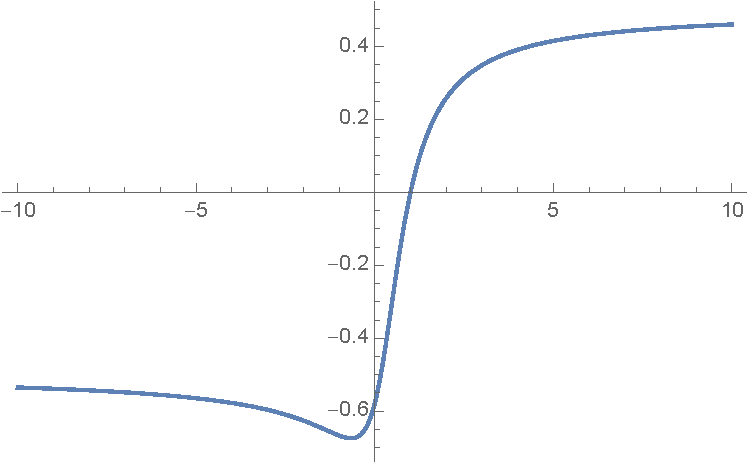
\includegraphics[scale = 0.7]{example01.pdf}
        \caption{$\lim_{x \to \infty} \frac{x - 1}{\sqrt{4x^2 - 2x + 3}}$}
        \label{fig:example01}
      \end{figure}

  \end{enumerate}

  \section{Difference of Infinite Quantities}

  \begin{align*}
    \lim_{x \to \infty} \sqrt{4x^2 + 1} - 2x & \neq \infty - \infty \\
    \\
    \lim_{x \to \infty} \sqrt{4x^2 + 1} - 2x & = \lim_{x \to \infty} \frac{1}{\sqrt{4x^2 + 1} + 2x} \\
      & = \lim_{x \to \infty} \frac{1/x}{\sqrt{4 + 1/x} + 2} \\
      & = \frac{0}{2 + 2} \\
      & = \boxed{ 0 } \\
  \end{align*}

  The two parts have to match exactly for the result to be zero:
  \begin{align*}
    \lim_{x \to \infty} \sqrt{4x^2 + 1} - 3x & = \lim_{x \to \infty} \frac{-5x^2 + 1}{\sqrt{4x^2 + 1} + 3x} \\
      & = \lim_{x \to \infty} \frac{-5 + 1/x^2}{\sqrt{4/x^2 + 1/x} + 3/x^2} \\
      & = \boxed{ -\infty } \\
  \end{align*}

  \newpage

  \section{Infinite Limits at Infinity}
  \begin{itemize}
    \item Only the highest degree exponent affects the limits as $x$ goes to $\pm \infty$

    \item Even powers behave like $f(x) = x^2$

    \item Even powers behave like $f(x) = x^3$

    \item As you zoom out, graph is indistinguishable from graph of just the leading term

    \item $f(x)$ gets larger and larger as $x$ gets larger and larger (or smaller and smaller)

    \item a rational function with degree of numerator larger than degree of denominator
      has $\pm \infty$ limit

  \end{itemize}

  \begin{figure}[H]
    \centering
    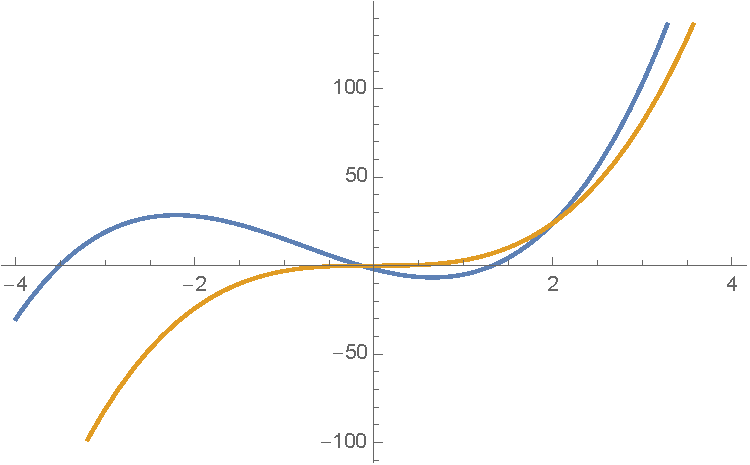
\includegraphics[scale = 0.6]{zoom01.pdf}
    \caption{$-4$ to $4$}
    \label{fig:zoom01}
  \end{figure}

  \begin{figure}[H]
    \centering
    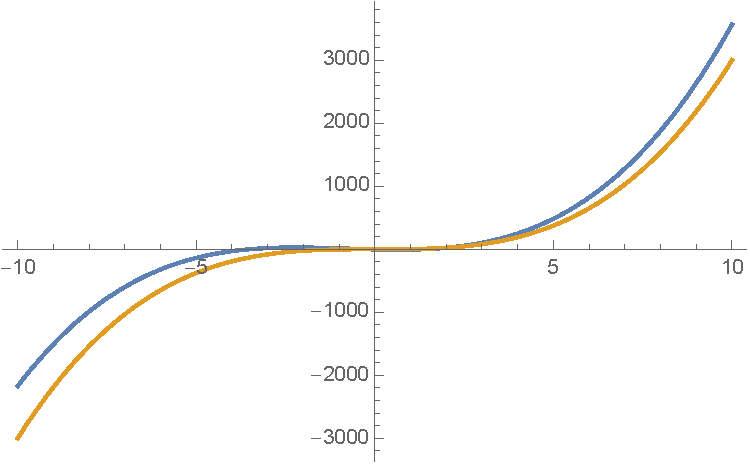
\includegraphics[scale = 0.6]{zoom02.pdf}
    \caption{$-10$ to $10$}
    \label{fig:zoom02}
  \end{figure}

  \begin{figure}[H]
    \centering
    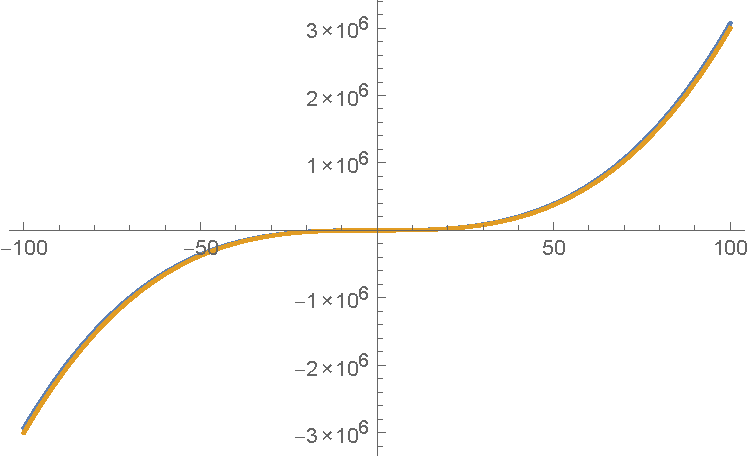
\includegraphics[scale = 0.6]{zoom03.pdf}
    \caption{$-100$ to $100$}
    \label{fig:zoom03}
  \end{figure}

  \section{Graphing}

  \begin{enumerate}
    \item 
      $f(x) = (x - 2)(x + 3)(x + 1)$ 
      \begin{figure}[H]
        \centering
        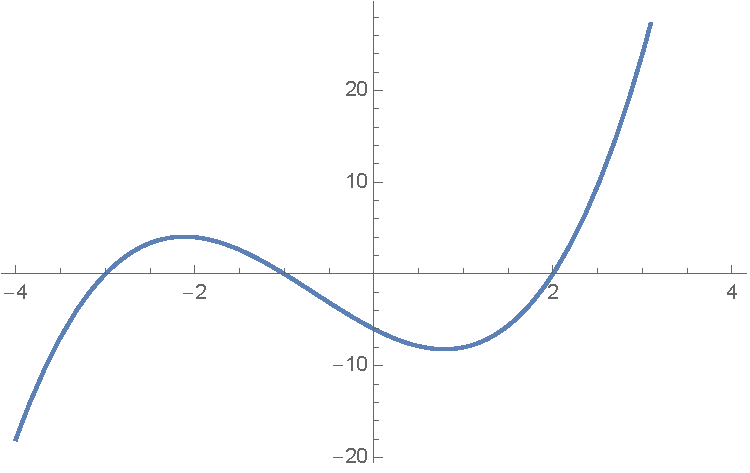
\includegraphics[scale = 0.6]{graphing01.pdf}
        \caption{$f(x) = (x - 2)(x + 3)(x + 1)$}
        \label{fig:graphing01}
      \end{figure}

    \item
      $f(x) = \frac{x^2-16}{x^2+x-6}$
      \begin{figure}[H]
        \centering
        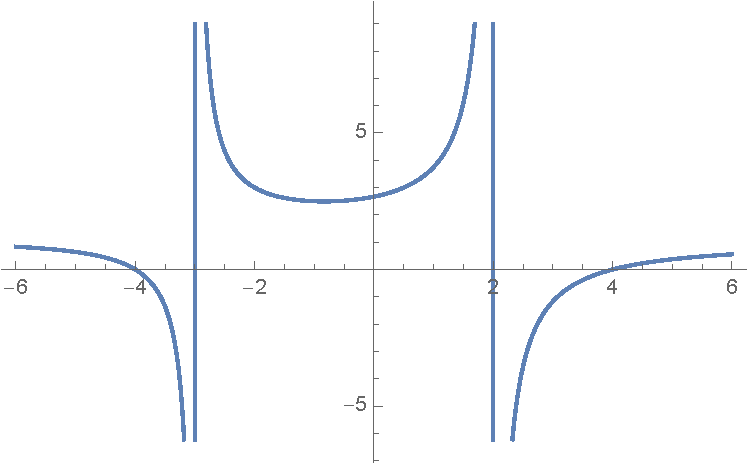
\includegraphics[scale = 0.6]{graphing02.pdf}
        \caption{$f(x) = \frac{x^2-16}{x^2+x-6}$}
        \label{fig:graphing02}
      \end{figure}
  \end{enumerate}

  \section{Precise Definitions}

  \subsection{Finite Limit}
  $\lim_{x \to \infty} f(x) = L$ means that for every $\epsilon > 0$ there is a corresponding
  $N$ such that if $x > N$ then $|f(x) - L| < \epsilon$.

  \subsection{Infinite Limit}
  $\lim_{x \to \infty} f(x) = \infty$ means that for every positive number $M$ there is a corresponding
  $N$ such that if $x > N$ then $f(x) > M$.

\end{document}

